\documentclass[11pt,a4paper]{article}
\usepackage[hyperref]{acl2020}
\usepackage{times}
\usepackage{latexsym}
\renewcommand{\UrlFont}{\ttfamily\small}

% This is not strictly necessary, and may be commented out,
% but it will improve the layout of the manuscript,
% and will typically save some space.
\usepackage{microtype}
\usepackage{tabularx}
\usepackage{multicol}
\usepackage{multirow}
\usepackage{afterpage,natbib,lipsum}
\usepackage{graphicx}
\usepackage{lipsum} 
\usepackage{tabulary}
\usepackage{subcaption}
\usepackage{booktabs}
\special{papersize=210mm,297mm}
\aclfinalcopy 
%\def\aclpaperid{***} %  Enter the acl Paper ID here

%\setlength\titlebox{5cm}
% You can expand the titlebox if you need extra space
% to show all the authors. Please do not make the titlebox
% smaller than 5cm (the original size); we will check this
% in the camera-ready version and ask you to change it back.

\newcommand\BibTeX{B\textsc{ib}\TeX}

\title{Hindi Poem Classifier}

\author{Abhishek Jaiswal 
  \qquad\quad
  Hardik Katyal
  \quad\quad
  Manan Gupta
  \qquad
  Mayank Wadhwani \\
  170101002   \quad\quad  \quad\quad 170101026 \quad\quad\quad\quad 170101035 \quad\quad\quad\quad 170101038\\ 
  Indian Institute of Technology Guwahati \\
  \textbf{Group No: 13}\\
  \url{https://github.com/mnk343/Hindi_Poem_Classifier}\\
  \{abhis170101002, katya170101026, manan170101035, mayan170101038\}@iitg.ac.in \\}

\date{\today}

\begin{document}
	
\maketitle
\begin{abstract}
\textbf{Poetic artistry} is a child of linguistic arts which, much like its siblings, visual and performing arts is heavily influenced by its creator and his ideology. Even in the greatest of masterpieces, we see the influence of the \textit{era} in which it was written materializing itself in subtle forms of expressions and vocabulary usages.
The works of \textit{Kabir}, one of the most well-known poets of Hindi, can be seen to be influenced by the \textit{Bhakti Movement}. He wrote most of his poems in vernacular Hindi frequently borrowing words from various dialects like \textit{Braj} encompassing topics like devotion, discipline, and mysticism.
All these intricate features including the use of beguiling metaphors, rhyme schemes, and the innate preference of an individual to a specific style of penmanship and vocabulary create an elaborate interplay almost akin to a fingerprint. These features can therefore be used for predicting the poet and era of previously unseen poems. This task has been effectuated for the English language but Indic languages like Hindi have largely remained untouched. We therefore propose to implement a model that handles this task for Hindi poems.
\end{abstract}


\section{Introduction}

\textit{T. S. Eliot} a leading poet of his times once said 
\begin{quote}
    \textit{"Genuine poetry can communicate before it is understood"}
\end{quote}

Poetry has been one of the oldest art forms known to mankind. It has been regarded as one of the noblest ones too with poets being adorned with the vaunted prizes by the most prosperous kings throughout the Indian history. One of the leading examples of this is one of the nine jewels of \textit{Akbar's} court, \textit{Tan Sen}. While all other genres are constricted by the shackles of plot, narration and need for grammatical consistency, poetry is free from all these restrictions. The words in a poem may not be used in their literal meaning and may have a deeper contextual connotation. 

\subsection{Motivation}
Poetry analysis in Indic languages has not received as much attention in recent years and this study is motivated towards starting that endeavour. Also the challenge that the level of ambiguity and subtlety that this problem provides as discussed previously provide a big motivation for us to tackle. 

\subsection{Objective \& Contribution}
 To this end, we start by creating a database of poems with the poet names and the era in which they were written and use this database to predict the poet and era for unseen samples. Our work can be used to classify computer generated poems towards the era and poets whose work it closely resembles. Also this project serves as a starting point for further exploration into the field of poetic analysis.

\section{Method}

The entire process has been divided into three major parts - \textbf{Dataset Creation}, \textbf{Data Cleaning and Preprocessing}, \textbf{Vectorization}, \textbf{Model For Prediction}.
\afterpage{
  \begin{figure}[t!]
    \centering
        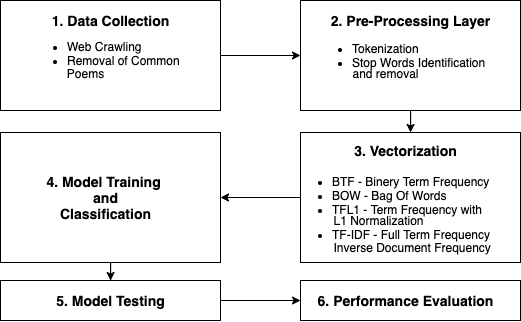
\includegraphics[width=\linewidth]{architecture2.png}
    \caption{Project Architecture}
    \label{fig:architecture}
  \end{figure}
}
\subsection{Dataset Creation}
The first step involved in poem classification is dataset creation. Since there is no corpus available publically we used web crawling on various sites, most prominently - \url{https://www.hindwi.org/poets} and \url{https://kavitakosh.org/}. Web crawler is a program that systematically browses the World Wide Web, typically for the purpose of web indexing. We used the web crawlers provided by the two libraries \textit{BeautifulSoup} and \textit{scrappy} in python.

Not all the sources provide the year in which the poem was written which makes it hard to assign the eras to the poem. The poems for which this information is unavailable, we use the date of birth of the poet as an estimate for the time of creation. This information is also missing for some poets, to circumvent this issue, we manually annotated the poets with the years they were active in. The final step is to assign eras to the poems on the basis of the year of their creation. We use the classification into eras as listed on \url{https://en.wikipedia.org/wiki/Hindi_literature}.

After collecting all the poems from all the various sources, we eliminate the duplicates from them using hashing. This gives us the final dataset that we split into a test set and a train set randomly  (90\%-10\% split). We have \textbf{45342} poems in our train set and \textbf{5038} poems in our test set.

\subsection{Data Cleaning and Preprocessing}
The second step in poem classification is data cleaning and preprocessing. For this we pass the poems through 2 sub-phases of text classification namely, tokenization and stop word removal. For tokenization we use \textbf{iNLTK} library which has pre-trained model for tokenization. Various punctiation marks like \textit{comma}(,), \textit{poorna viram}($|$) and \textit{exclamation mark}(!) among other are commonly occurring symbols in the poems, therefore we further go on to remove the various stop words from the tokenized output. The stop words have been collected from various sources -
\url{https://data.mendeley.com/datasets/bsr3frvvjc/1}, \url{https://sites.google.com/site/kevinbouge/stopwords-lists},  \url{https://github.com/taranjeet/hindi-tokenizer/blob/master/stopwords.txt}.

\begin{table*}[htb!]
\setlength\tabcolsep{0pt}
\smallskip 
\begin{tabular*}{\textwidth}{@{\extracolsep{\fill}}cccc}
\toprule
  \textbf{Model}  & \textbf{Vectorization Technique} & \textbf{Poet Accuracy} & \textbf{Era Accuracy} \\
\midrule
  \multirow{4}{*}{\textit{Cosine Similarity}} & \textit{BTF}   & 16.435\%    &  87.594\%    \\
   & \textit{BoW}   & 11.572\%    &  83.287\%    \\
   & \textit{TFL1}   & 11.572\%    &  83.287\%    \\
   & \textit{TF-IDF}   & 12.584\%    &  84.021\%    \\
  \midrule
  \multirow{4}{4cm}{\centering\textit{Logistic Regression (Random Search)}} & \textit{BTF}   & \textbf{32.115\%}    &  89.261\%    \\
   & \textit{BoW}   & 16.633\%    &  88.298\%    \\
   & \textit{TFL1}   & 3.655\%    &  88.314\%    \\
   & \textit{TF-IDF}   & 23.322\%    &  89.380\%    \\
  \midrule
  \multirow{4}{3.5cm}{\centering\textit{Logistic Regression (Grid Search)}} & \textit{BTF}   & 31.044\%    &  \textbf{89.718\%}    \\
   & \textit{BoW}   & 16.613\%    &  88.427\%    \\
   & \textit{TFL1}   & 3.751\%    &  88.527\%    \\
   & \textit{TF-IDF}   & 24.612\%    &  89.559\%    \\
\bottomrule
\end{tabular*}
\caption{Accuracy of Different Models and Vectorization Methods on the Test Set} \label{results}
\end{table*}

\subsection{Vectorization}
The third step in poem classification is vectorization. The preprocessed data obtained from the second step needs to be converted into a format which can be later used by different models. We use different vectorization techniques to accomplish this. More formally, we convert the text into numerical representation by using several different techniques. 
\begin{enumerate}
    \item \textbf{BTF} or \textbf{Binary Term Frequency} captures the presence (1) or absence (0) of a term in a document.
    \vspace{-0.2cm}\item \textbf{BoW} or \textbf{Bag Of Words} Term Frequency is used to assign the exact frequency of a term instead of just classifying it into 1 or 0 as done in the BTF technique.
    \vspace{-0.2cm}\item \textbf{TFL1} or the \textbf{L1 Normalized Term Frequency} is a technique which applies L1 normalization on the BoW term frequency in the document.
    \vspace{-0.2cm}\item \textbf{TF-IDF} or \textbf{Term Frequency-Inverse Document Frequency} also takes into account the distinctness of a term in a document along with its frequency. So if a term is present in few documents, then the corresponding TF-IDF value is expected to be higher than otherwise.
\end{enumerate}
These different vectorization techniques were applied by passing appropriate parameters to the \textit{TfidfVectorizer} included in the \textit{sklearn (sci-kit learn)} package in python.

\subsection{Model Training and Testing}
The fourth step in poem classification is model training and testing. At the end of the third stage we have the representation of the poems data as vectors. We now test different NLP and ML based models for the task of classification with all the different vectorization methods explained previously. We have used appropriate functions from the \textit{sklearn} package in python to implement the various models. We now briefly explain all the different models that we have explored in the course of this project.

\begin{enumerate}
    \item \textbf{Cosine Similarity} is a NLP based metric used to quantify the similarity between different documents. Mathematically, it finds the dot product of the documents represented as vectors in a multi-dimensional space. Given a poem, we try to find the most similar poem from the training set (which has the highest value of cosine similarity) and then return the corresponding era and the poet name. 
    
    \item \textbf{Logistic Regression} is one of the most powerful tools in statistical modeling which we use directly on the input vectors. We make use of the \textit{numpy} package for intermediate output representation. We have used various search techniques provided in these libraries for tuning the hyper-parameters including \textit{RandomizedSearchCV} and \textit{GridSearchCV}. We only report the best among all the results that we obtained from all of these search techniques.
    
    \item \textbf{Convolutional Neural Network} method is very similar to ordinary Neural Network. It is made of neurons that have learnable weights and biases. Each neuron receives some inputs, performs a dot product and optionally follows it with a non-linearity. The whole network expresses a single differentiable score function: from the raw vectorized input on one end to class scores at the other. And it has a loss function on the last (fully-connected) layer.
    
\end{enumerate}

\section{Progress}
We have been able to entirely complete the first 3 steps namely dataset creation, data cleaning and preprocessing and vectorization. We have also implemented and found the results for 2 of the 3 proposed models in the above section - \textit{Cosine Similarity} and \textit{Logistic Regression}.

\section{Results}
Table~\ref{results} shows the accuracy of different models with different vectorization techniques on the test set for both poet prediction and era prediction. The best result obtained for era prediction had an accuracy of \textbf{89.718\%} and for poet prediction \textbf{32.115\%}. There are multiple reasons why we do not see as good results for poet prediction as we see for era prediction, the most prominent being that the number of poets to be predicted is much larger than the number of eras. Also because we have used a random split for test set creation, there are cases were the poet in the test set is not part of train set altogether. This makes it impossible for any model to give a correct result on these examples. This however shows the power of deduction of the era as even in the cases where we do not have any poem from a poet in the test set, the era is predicted with high accuracy. Also the vectorization methods used gave long and sparse vectors which made training the models a difficult task and we were forced to run lower number of iterations of the optimization algorithm because of time constraints. Hence, the trained model might not be the most optimal one. We also present the results in a graphic format in Figure~\ref{histogram}.

\begin{figure*}[htb!]
    \centering
    \begin{subfigure}{.5\textwidth}
      \centering
      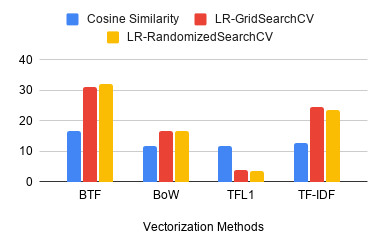
\includegraphics[width=\linewidth]{Poet.png}
      \caption{Poet Accuracy}
      \label{fig:sub1}
    \end{subfigure}%
    \begin{subfigure}{.5\textwidth}
      \centering
      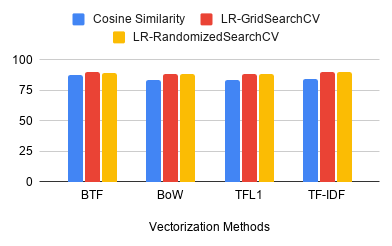
\includegraphics[width=\linewidth]{Era.png}
      \caption{Era Accuracy}
      \label{fig:sub2}
    \end{subfigure}
    \caption{Accuracy of Different Models and Vectorization Methods} 
    \label{histogram}
\end{figure*}

\section{Future Works}
We wish to complete the evaluation of the CNN model as well as proposed earlier. We hope it will be able to learn a more accurate decision boundary than the logistic regression method and therefore imporove our results. We would also like to explore different vectorization techniques that give short and dense vectors which may help in training our models in the last step much faster and feasible.

\section{Conclusion}
In this work, we compare different approaches for determining era and poets of Hindi poems. The vectorization was done using 4 methods, namely Binary Term Frequency, Bag of Words, (L1) Normalised Term Frequency \& (L2) Normalised TF-IDF. The models used were Cosine Similarity and Logistic Regression among others. 

This work also serves the evaluation of poems whose sources are not known. Logistic models perform better than cosine similarity based models on the datasets considered  in  this  paper so far. 

This project explores new dimensions by improving the quality of Poem Classification for Hindi Language and hopes to generate more effort in this domain. 

\vspace{6cm}
\nocite{c1}
\nocite{c2}
\nocite{c3}
\bibliography{acl2020}
\bibliographystyle{acl_natbib}

\end{document}
